\chapter{EcoBuilder}
\label{chap:joy}

\begin{figure}
    \centering
    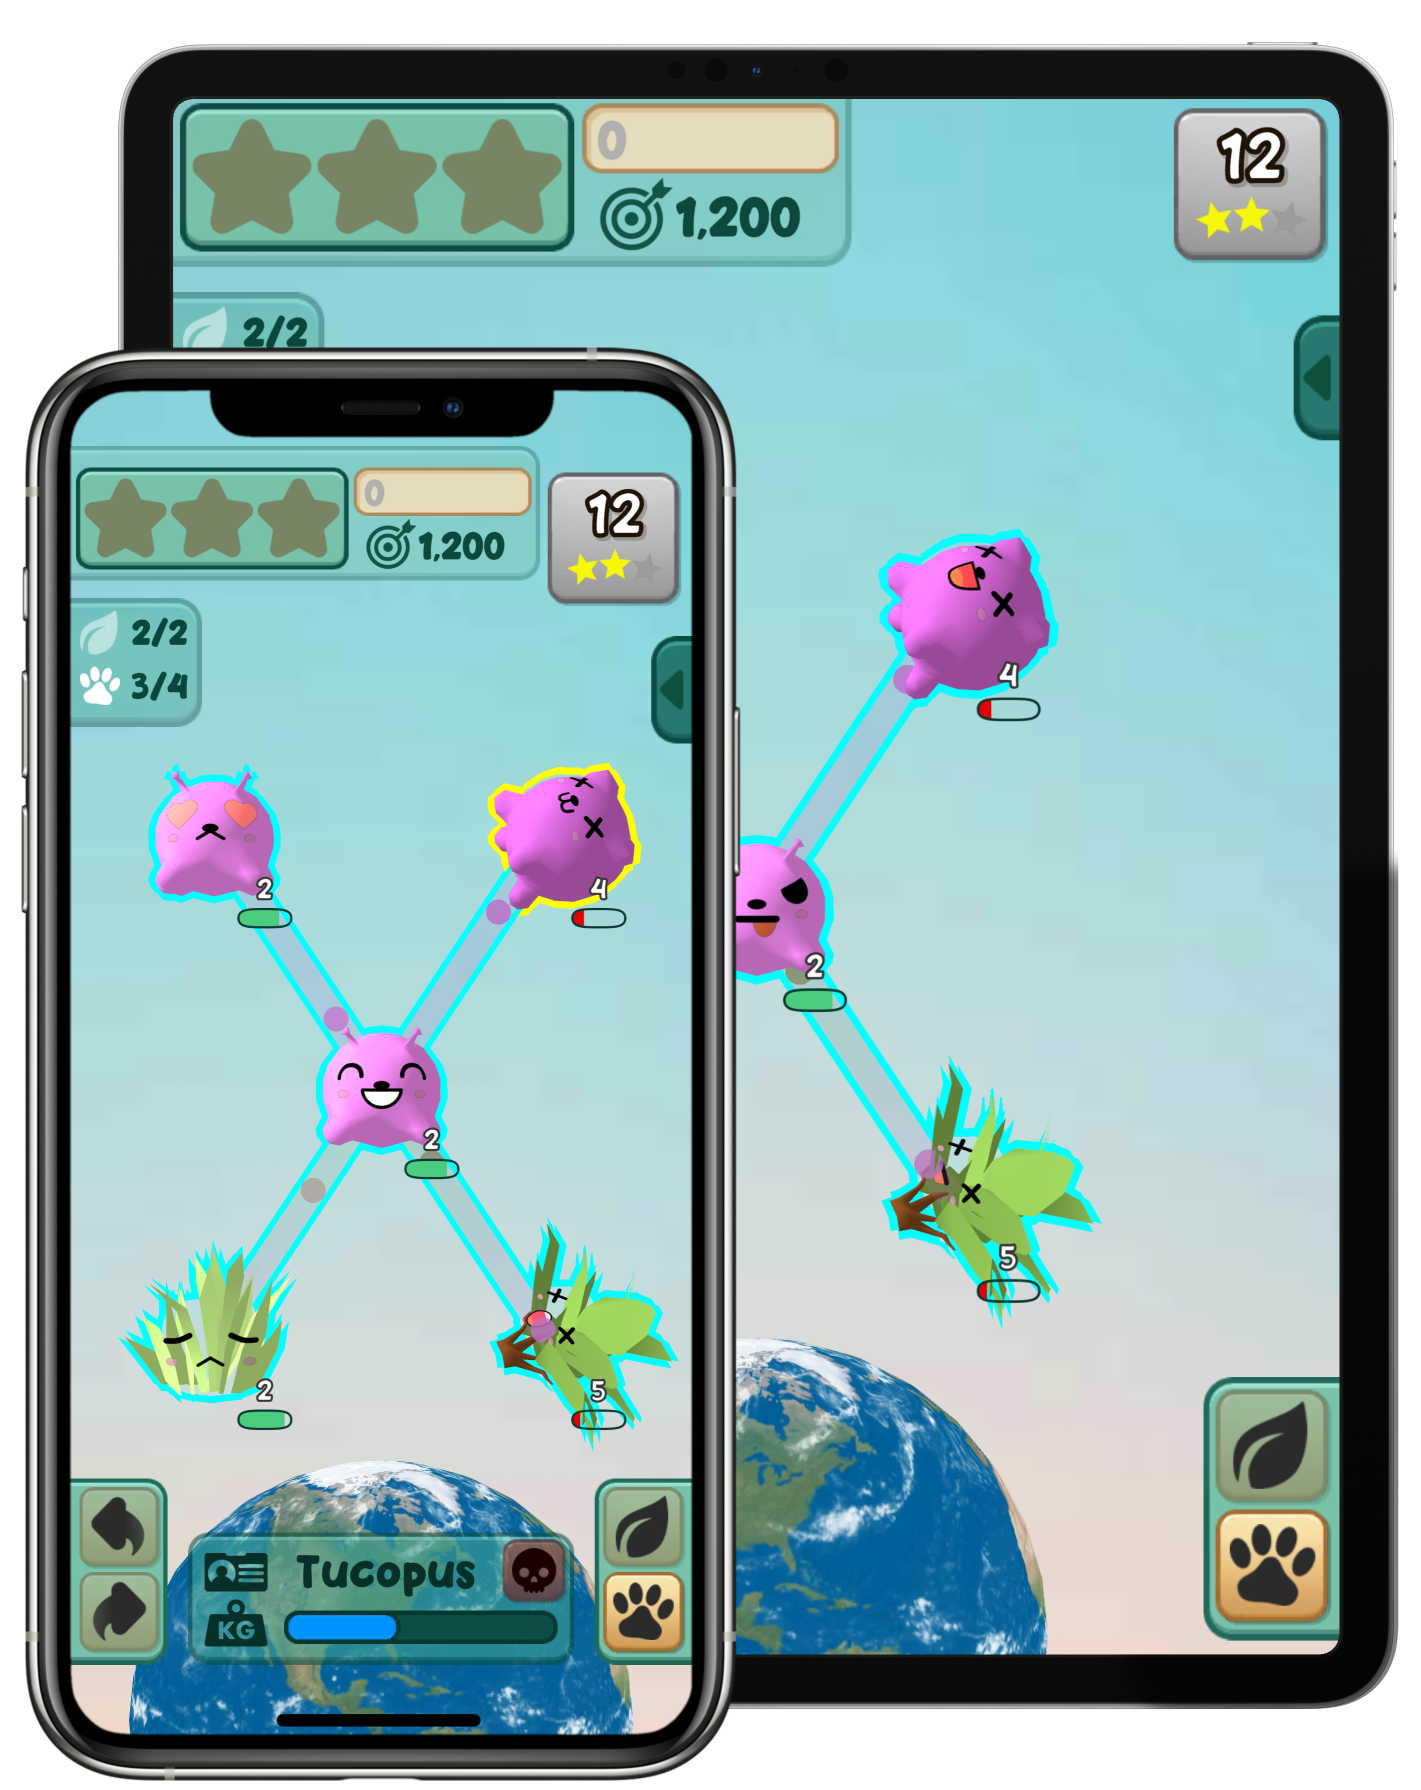
\includegraphics[width=\textwidth]{joy/device.png}
    \caption[A screenshot of EcoBuilder displayed on mobile devices.]{A screenshot of EcoBuilder displayed on two mobile devices. The particular ecosystem shown depicts the bottom-right plant going extinct due to apparent competition, as well as the top-right animal going extinct due to competitive exclusion.}
    \label{fig:my_label}
\end{figure}

The preceding chapters focused on the algorithms and methods underlying visualisation techniques, but it is important to remember that visualisation is a discipline with practical applications firmly in mind as the end goal.
The work in this chapter will explore such a goal to move towards an engineering focus, specifically the design and development of \emph{EcoBuilder}, a research-oriented video game about building ecosystems.

\section{Background}
\label{sec:joy_background}
The unique selling point of EcoBuilder is that its ecosystem simulation is based on the same mathematical models studied by theoretical ecologists. The review of background literature in this section will therefore begin by discussing the models chosen in the following Section~\ref{sec:predator_prey}. With the knowledge of \emph{how} a pair of species interact with each other, the following Section~\ref{sec:topology} will study the choice of \emph{which} species interact at all. A final background Section~\ref{sec:citizen_science} will outline a brief history of previous attempts to crowdsource research through the citizen science approach.

\subsection{Predator--prey interactions}
\label{sec:predator_prey}
Ever since Isaac Newton formulated his physical laws of motion, it has become clear that nature speaks in the language of differential equations. From simple mechanical systems such as the oscillating swing of a pendulum \cite{Fulcher1987}, to the cosmic dance of celestial bodies in space \cite{Marchal2012}, and even the electrical action potentials across every neuron in the brain deciding which words should go into this sentence \cite{Hodgkin1952}, calculus has time and again been an invaluable tool for describing the natural world. 

The behaviour of species ecosystems is no different, where the most widely used models are function by defining the change in population over time.
There are many such examples of this, ranging from the simple and linear systems to be studied here, to highly complex data-driven models such as \emph{EcoPath with EcoSim} which has been used for decades to inform environmental policy for aquatic conservation \cite{Christensen2004}.
Models that include the effects of temperature \cite{Savage}, species migration \cite{SpacialTemporal}, or evolution \cite{TangledWeb}

But perhaps the oldest and most commonly studied of these models is known as the Lotka-Volterra equations, defined as
\begin{equation}
  \frac{d\mathbf{x}_i}{dt} = \mathbf{x}_i(\mathbf{r}_i + \sum_j\mathbf{A}_{ij}\mathbf{x}_j)
  \label{eq:lotka_volterra}
\end{equation}
where $\mathbf{x}_i$ is the population of species $i$, $\mathbf{r}_i$ is its growth rate (or death rate if it is negative), and $\mathbf{A}_{ij}$ is the strength of the interaction between two species, which is positive if $j$ is a resource of $i$ or negative if $j$ is a consumer of $i$. 
This can be written in include all species simultaneously as
\begin{equation}
    \frac{d\mathbf{x}}{dt} = \mathbf{x}(\mathbf{r} + \mathbf{Ax}).
    \label{eq:interaction_matrix}
\end{equation}
The matrix $\mathbf{A}$ is known as the \emph{interaction matrix}, and is called that because it contains all the information on how each pair of species interact with each other.
There are five classifications of interaction possible in such a model, designated by the nature of the values in the corresponding pair of values in this matrix. For example, if $\mathbf{A}_{ij}>0$ and $\mathbf{A}_{ji}<0$, then it is a standard example of species $i$ preying on species $j$, where the `sign' of the interaction is $(+,-)$. The remaining types are mutualism $(+,+)$, competition $(-,-)$, commensalism $(+,0)$, and amensalism $(-,0)$.
Different models include differing amounts of each type of interaction, and the proportion of types can strongly influence the behaviour of the system \cite{Tang2014}. However the predator--prey type is the most commonly studied and most prevalent in nature \cite{TODO} and so will be the only one considered here.

The purpose of the above equations is to use them to find values of $\mathbf{x}$, and the standard way of doing this for differential equations is to simulate by performing numerical integration at each time step, using methods such as Runge-Kutta \cite{TODO}.\footnote{this was what was done in older versions of the game, but brings with it a number of problems, such as stiff equations leading to instability \cite{TODO}, or having to choose an integration time step or extinction threshold as input parameters.}
However the simplicity of the model chosen allows something different: it can be analytically solved for an \emph{equilibrium} point. This is the solution at which the interactions fully balance each other such that the instantaneous change in population is zero. Note the similarity of this method to the graph layout algorithm of Tutte shown in Section~\ref{sec:nodes_background}, Equation~\eqref{eq:tutte}.
This is done by setting the left-hand side of Equation~\eqref{eq:interaction_matrix} to zero, where it is clear that the system contains many trivial solutions with any species $x=0$, which corresponds to the natural case of an extinct species staying extinct.
Since the solution at which every species has non-zero population is one of interest, the $\mathbf{x}$ outside bracket is simply cancelled out to reach the solution
\begin{equation}
  \mathbf{x^*} = -\mathbf{A}^{-1}\mathbf{r}.
  \label{eq:equilibrium}
\end{equation}
where $\mathbf{x}^*$ is the strictly non-zero populations of every species at equilibrium.
This is equivalent to a linear system of equations and so can be solved exactly by numerical methods.
If the solution $\mathbf{x^*}$ contains any negative numbers the system of equations is said to not be \emph{feasible} i.e.\ it is not possible for all species to coexist.

\subsubsection{Local asymptotic stability}
If the system is feasible, another benefit of this technique is that it allows for the derivation of the \emph{local asymptotic stability} of this fixed point, which has been widely used in the literature as a mathematically elegant and computationally tractable measure of the `health' of food webs~\cite{May1973, Emmerson2004}. This local stability will be henceforth referred to simply as stabllity. 
To do this the first step is to find the Jacobian matrix
\begin{equation}
  \mathbb{J} = \begin{bmatrix}
    \frac{\partial f_1}{\partial \mathbf{x}_1} & 
    \cdots &
    \frac{\partial f_1}{\partial \mathbf{x}_n} \\
    \vdots &
    \ddots &
    \vdots \\
    \frac{\partial f_n}{\partial \mathbf{x}_1} & 
    \cdots &
    \frac{\partial f_n}{\partial \mathbf{x}_n}
  \end{bmatrix}
\end{equation}
where $f_i$ is the right side of Equation~\eqref{eq:lotka_volterra} and $n$ is the total number of species in the food web.
This is the matrix of all possible partial derivatives of a system, which describes the instantaneous behaviour of the system by linearising it. This Jacobian is then evaluated at the feasible equilibrium point $\mathbf{x}^*$, resulting in the \emph{community matrix}. For the Lotka-Volterra equations studied here, this is
\begin{equation}
  \mathbb{J}|_\mathbf{x^*} = \begin{bmatrix}
    \mathbf{r}_1 + 2\mathbf{A}_{11}\mathbf{x}_1^* + \sum_{i\neq 1}^n\mathbf{A}_{1i}\mathbf{x}_i^*
    \;\cdots\;
    \mathbf{A}_{1n}\mathbf{x}_1^*\\
    \vdots 
    \qquad\qquad\quad\;\;\ddots\qquad\qquad\quad\;\;
    \vdots \\
    \mathbf{A}_{n1}\mathbf{x}_n^*
    \;\cdots\;
    \mathbf{r}_n + 2\mathbf{A}_{nn}\mathbf{x}_n^* + \sum_{i\neq n}^n\mathbf{A}_{ni}\mathbf{x}_i^* 
  \end{bmatrix}
  \label{eq:jacobian_evaluated}
\end{equation}
which can also be simplified to $\mathbb{J}|_\mathbf{x^*} = \mathbf{Ax*}$ using Cramer's rule \cite{TODO}.
The system can then be declared locally stable if the largest real part of any eigenvalue of the community matrix is non-negative
\begin{equation}
    \Lambda \leq 0.
    \label{eq:lambda_stability}
\end{equation}
% In fact the further away from zero $\Lambda$ is, the quicker the system returns to the equilibrium point $\mathbf{x}^*$ after a perturbation, and therefore the more resilient the ecosystem is.
An intuitive physical interpretation of this type of stability can be seen by imagining the two ways of holding a chopstick vertically when gripping only a single end. If the chopstick is pointing upwards, even the slightest nudge will make it fall over due to gravity. If it is dangling downwards, gravity will reset its position after a nudge, and it can be called stable.
In the context of ecosystems, the chopstick is a species, and the nudge is an environmental perturbation such as a natural disaster or invading species.

The behaviour of the community matrix $\mathbb{J}|_\mathbf{x^*}$ is what is usually studied in mathematical ecology, due to the fact that it can be reverse engineered to apply to any system of differential equations. It therefore sidesteps the problem of choosing which model to use, by jumping straight to this matrix.
It is also the source of the long standing `complexity vs.\ stability' debate in the world of ecology, because it can be shown that as the number of species, i.e.\ size of $\mathbf{A}$, grows, the chance of Equation~\eqref{eq:lambda_stability} being satisfied tends to zero, even for small ecosystems of only a few dozen species \cite{May1973}.
The reason for the debate is that systems exist in the real world with many more species than the math suggests is possible, and many subsequent works have studied what features of ecosystems allow such a contradiction to occur \cite{Tang2014, brose, samjohnson}.

However a common criticism is the assumption of the existence of a feasible equilibrium in the first place, and this is far from guaranteed \cite{TODO}. It has also been showed that in simple systems like the Lotka-Volterra equations studied here, that feasibility almost always leads to stability anyway \cite{Dougoud2018}. For this reason, the work done here will focus solely on feasibility, where nevertheless any results found can also apply to stability.

% We plan on using \eqref{eq:lambda_stability} directly within the game as one of the possible metrics for a high-score.
% Other possible metrics include the total energy flow (flux) of the system, the trophic height (largest trophic level), or the reactivity of the fixed point~\cite{Tang2014}.
% All of the three solutions just described have been implemented into the game and an early screenshot can be seen in Figure~\ref{screenshot}.

% As we shall see, this also solves our issue of having to choose a suitable extinction threshold, as well as having to integrate differential equations for a long time after the game ends to make sure that species slowly on their way to extinction do not count towards the player score.


\subsubsection{Metabolic scaling}
The steps so far have discussed how to find populations given the interaction matrix $\mathbf{A}$, but it has not yet been discussed how to find the numerical values to go into the matrix in the first place, i.e.\ its parameterisation.
To fill this gap, a methodology known as \emph{metabolic scaling} will be used. It leverages the idea that the metabolism of a species, i.e.\ the speed at which an organism converts a food source into either energy for movement or materials for growth. For plants this involves mainly converting nutrients and sunlight into biomass, and for animals this involves mainly converting biomass into movement to hunt prey.

\begin{figure}
    % \centering
    % \includegraphics{}
    \caption[metabolism]{show metabolism against size if you can}
    \label{fig:my_label}
\end{figure}

Metabolism is useful for two main reasons. The first is that, as it essentially measures the energy output of a species, it is strongly correlated with other traits such as movement speed \cite{Hirt2017} and therefore has been successfully used for parameterisation of $\mathbf{A}$ \cite{Brosespeed, Brose, Pawar}. The second is that metabolism can be estimated very closely through its relationship to body size, which can be measured and verified simply with a set of scales \cite{Brose}.
Specifically, the parameters required for reproduction rates in Equation~\eqref{eq:lotka_volterra} are
\begin{equation}
  \mathbf{r}_i =
  \begin{cases}
    \;b_0\mathbf{m}_i^{\text{--}\sfrac{3}{4}} & \text{if $i$ is producer}\\
    \;-d_0\mathbf{m}_i^{\text{--}\sfrac{3}{4}} & \text{if $i$ is consumer}
  \end{cases}
\end{equation}
where $b_0$ and $d_0$ are constants measuring birth and death rates, and $\mathbf{m}_i$ is the body mass of species $i$ in kilograms. This relationship has been empirically verified by many sources \cite{Brose, Gillooly}.
The interaction strengths of a predator--prey reaction are defined as
\begin{equation}
  \mathbf{A}_{ij} =
  \begin{cases}
    \;-a_0\mathbf{m}_j^{\text{--}\sfrac{3}{4}} & \text{if $i$ is prey}\\
    \;\;\,e_0a_0\mathbf{m}_i^{\text{--}\sfrac{3}{4}} & \text{if $i$ is predator}
  \end{cases}
\end{equation}
where the values of $a_0$ and $e$ are constants measuring search rate and biomass conversion efficiency. This relationship is more difficult to empirically verify as it involves measuring gut content as a surrogate for interaction, but has been used successfully for many studies. Note that the subscripts for interaction strength always only depend on the mass of the predator, as it is the predator that is doing the foraging.

This model of a predator--prey interaction has been criticised in the past for being too simplistic, and more complex models such as Type II or III functional responses \cite{Holling1973} have introduced non-linear functions into $\mathbf{A}$ in order to capture the effects of handling time and satiation, respectively.
% Despite their increased realism and accuracy, it was decided to only consider a linear functional response here.
% However it is possible to endlessly parameterise any model of the natural world, and even though more complex models do lead to more accurate results
However, due to the added complexity to the model and the fact that the equilibrium calculation in Equation~\eqref{eq:equilibrium} would become much more difficult due to a non-linearity, it was decided that only a linear functional response will be considered here.
Additionally, the equations above only require a single varying parameter of species mass, in order to parameterise every single value in the system. That is, except for the diagonal values of $\mathbf{A}$, which will be discussed in the following section.

\subsubsection{Intraspecific interference}
It is well known that no species can grow exponentially forever, as there is always some point at which the population of any species reaches its carrying capacity. 
% This is because exponential growth is almost always logistic growth in disguise
This applies to almost every example of exponential growth in the real world, from the growth of a business on the stock market, to the spread of a deadly virus.

This is captured by the diagonal elements of the interaction matrix $\mathbf{A}_{ii}$. This can be interpreted as the amount that species interacts with itself, or in other words the \emph{intraspecific interference}. It is always a negative value, because otherwise the population of a species would grow even faster than exponentially, and can be interpreted as competition between individuals over space.

This value has a strong effect on the dynamics of the model. In fact, it can be shown that any ecosystem can be made stable by simply increasing the magnitude of the diagonal values of the community matrix in Equation~\eqref{eq:jacobian_evaluated}. 
Barab\'as et al.\ \cite{Barabas2017} further showed the importance of these values, as they proved that it only takes one weak interference value to spoil the stability of an entire ecosystem.

Unfortunately, there is no easy way to measure this value in real world ecosystems, as quantifying the amount a species competes with itself is difficult. Previous works have overcome this problem by assuming every species can coexist at a population following Damuth's law, which states that the species with larger body sizes tend to have smaller overall populations. The values for $\mathbf{A}_{ii}$ are then calculated for these populations, and used as a proxy for the health of an ecosystem \cite{Pawar}. However this is the opposite order of causation, as the behaviour of $\mathbf{A}$ should be the mechanism underlying Damuth's law in the first place.

Without a good way of deriving these diagonal values, the work in this chapter will simply leave them as another input parameter. The interference of each species, alongside the body mass to parameterise the off-diagonals as in the previous section, will therefore be free parameters for the work done here.

% values following Hsi-Cheng were chosen for a\_ii
% chicken and egg problem: either pick abundances with damuth's law measure a\_ii, or pick a\_ii and then find feasibility. WTF

\subsection{Food web topology}
\label{sec:topology}
The final missing piece from the model needed to finally simulate an ecosystem is simple: deciding which species should interact with each other at all.
This study of this topology of food webs has seen many models being developed to capture the non-randomness that exists in their structure.

One of the main features that such models attempt to capture is the idea that big things generally eat small things. An early version of this is the cascade model by Cohen \cite{Cohen}, which gives begins by placing every species along an axis, and then only allows species to prey on other species that are lower than them on this axis. The placement on this axis can, but is not necessarily, interpreted as body size.
A notable improvement to this is the Niche model of Williams and Martinez \cite{Williams2000}, who leveraged the fact that big things eat small things, but not too small. They therefore constrained species to only prey on other species on a certain range on the axis.
Other attempts include the nested hierarchy model \cite{TODO} which captures the clustered nature of food webs, the coherence model \cite{Johnson} which captures the layered nature of groups of predators, or the speciation model \cite{Rossberg2006} which simulates evolutionary processes to produce structure as an emergent property.

However, none of these models can capture the topology of food webs fully satisfactorily. Furthermore, thinking about the options to give a player, it would be much more interesting to have full control over what interactions exist. That is the choice used from this point on, but a good question to ask at this point is whether it is possible for humans to comprehend the topology of real world webs.

\subsubsection{Dimensionality}
One thing that all the aforementioned models share is \emph{low dimensionality}. This essentially means that there exists a structural pattern that can be largely explained using rules and models without too many parameters.
% The models described have been shown to recreate ecosystem features well, but is there a way to quantify whether real food webs can even be described with models without too many parameters?
% The second critical flaw of the game was the fact that the user had no control over the structure of the food webs they were creating.
It is important that the dimensionality of topologies players are tasked with recreating is low, because humans struggle with understanding high-dimensional information. After all, the algorithms studied in previous chapters all aimed at reducing the dimensionality of graphs down to two dimensions. To gain an idea of just how complicated structures can become, the number of possible edges in a directed graph is $n(n-1)$, which means that there are $2^{n(n-1)})$ possible configurations for the user to try, assuming edges can go in both directions. Even if edges can only in one direction then there are $3^{n(n-1)/2}$, which is still worse than exponential. To illustrate how fast this grows, just six species already means over 10 million possible topologies.

It may then seem impossible for the player to effectively explore this search space, but low-dimensional topologies should mean that simple strategies and patterns can be used to successfully construct them.
Fortunately, a study by Eklof et al.\ \cite{Eklof2013} collected a massive amount of empirical data and directly asked the question of what dimensionality empirical food webs exhibit. Dimensionality in this case is defined as the number of \emph{niche axis} required to capture the topology of a food web, which follows the same definition as the aforementioned niche model. An example of this is shown in Figure~\ref{fig:niche}.

\begin{figure}
%   \centering
%   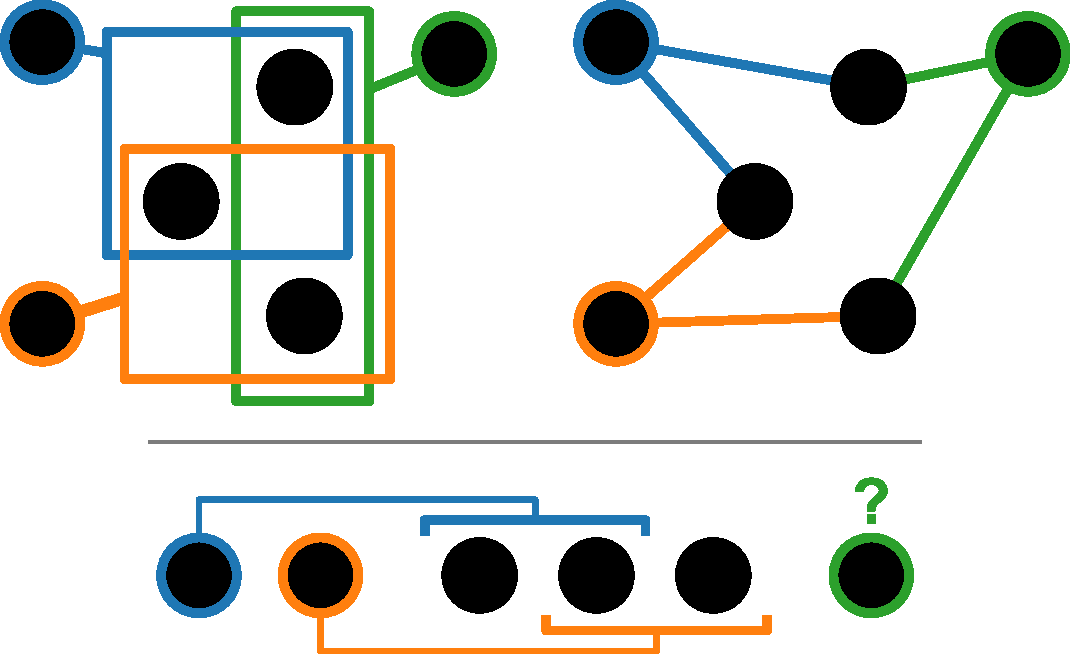
\includegraphics[width=.8\linewidth]{niche.pdf}
  \caption{Example of a 1D niche structure (top) and 2D (bottom), with a consumer and its feeding range in red, and resources in green.
  In one dimension it is not possible to eat only the left and right species, but given another dimension it is possible for the middle species to `escape'.}
  \label{fig:niche}
\end{figure}

Eklof et al.\ \cite{Eklof2013} searched for the minimum number of niche axis required, by applying an algorithm that searches the space by swapping certain species one by one, and then estimating the `best' dimension using the Akaike information criterion \cite{Eklof2013}. This is necessary because there does not exist a polynomial time algorithm for determining the number of axis required.
Their result was that the number of dimensions needed to describe even the largest webs is surprisingly low. For smaller webs (fewer than 250 interactions) only one dimension was needed, and only four were needed for their best prediction on webs with thousands of species (with a mean of 1.395 over all webs).
This means that simple strategies and patterns should be able to describe any real food web topology, and therefore that humans can hope to form such strategies.

\subsubsection{Trophic levels}
A final topological feature that will be considered is the \emph{trophic level} of each species, specifically the prey-averaged trophic level \cite{Williams2004}, defined as
\begin{equation}
  t_j = 1 + \sum_i^n p_{ij}t_i
\end{equation}
where $p_{ij}$ is the proportion of the diet of $j$ that $i$ contributes to. This essentially means that the trophic level of a species is equal to the average trophic level of its prey plus one.
The similarity of this definition to Tutte's algorithm back in Chapter~\ref{chap:stress}, Equation~\eqref{eq:tutte} is worth noting, as the matrix solved here is also a graph laplacian.

This can be solved by moving the summation to the other side and converting it into a system of linear equations
\begin{equation}
    \begin{bmatrix}
    1&-p_{2,1}&\cdots&-p_{n,1}\\
    -p_{1,2}&1&\cdots&-p_{n,2}\\
    \vdots&\vdots&\ddots&\vdots\\
    -p_{1,n}&-p_{2,n}&\cdots&1
    \end{bmatrix}
    \begin{bmatrix}
    t_1\\t_2\\\vdots\\t_n
    \end{bmatrix}
    =
    \begin{bmatrix}
    1\\1\\\vdots\\1
    \end{bmatrix}
\end{equation}
where most of the values of $p_{ij}$ will be zero because the structure will be reasonably sparse.
The matrix also has the nice property of being diagonally dominant, which means that iterative methods such as Gauss-Seidel are guaranteed to converge~\cite{Young2014}. This will be made use of later in Section~\ref{sec:eco_visualisation}.

It is widely accepted that the trophic level of species has a deep meaning within the context of ecosystems~\cite{Post2002}. This is because species with high trophic levels tend to be more biologically complex, as they are at the top of the food chain, like humans for example. Trophic level will therefore be made use of in Section~\ref{sec:eco_visualisation} within a visualisation context.

\subsection{Citizen science}
\label{sec:citizen_science}

At the time of writing, video games have grown large enough to eclipse the film and music industries, combined \cite{Egenfeldt-Nielsen2019}. Its recent growth is due to the rise in mobile and competitive gaming, which have been a rounded out the market to appeal to casual and hardcore audiences respectively.
% https://www.ejinsight.com/eji/article/id/2280405/20191022-video-game-industry-silently-taking-over-entertainment-world

Their popularity has also spilled into the world of research, with a variety of research-oriented games being produced in a range of disciplines. The motivation behind making such games is twofold, as they can simultaneously perform outreach through public engagement, as well as real research through crowdsourcing of human intelligence.

This crowdsourcing is known as \emph{citizen science}, and is not limited to the digital world; it has been successfully applied to things like soil...
Even in the digital space, citizen science does not necessarily require a gamified context in order to perform the crowdsourcing. One of the oldest digital citizen science projects is \emph{Galaxy Zoo}, \cite{Ponti2018}
In the context of on problems that computers cannot handle.
The most successful examples of this include:
\begin{itemize}
  \item \emph{Foldit}
  \item \emph{Eyewire}
  \item \emph{EteRNA}
  \item \emph{fold.it}
\end{itemize}
It has evenborderlands minigame etc.

This is cool. How it will be attempted will be described in the following section.

\section{Design and Hypotheses}
based around simulating the species ecosystems underlying the nature all around us.

This chapter will therefore contain...

\subsection{Visualisation}
\label{sec:eco_visualisation}
\subsubsection{TROPHIC LEVELS}
\begin{itemize}
  \item gauss-seidel iteration because positive definite, optimised to only take O(m) per iteration and O(n) extra space (because we only care about the sum of the rows and not where the rows are placed. In general we find the number of iterations required is <100 (test this) but requires for loops
  \item whether this laplacian has a solution can also be found using a breadth first search from sources (which is also used for chain)
  \item note that this is the same set of equations as in \eqref{eq:tutte} and \eqref{eq:major_Lw}, \eqref{eq:major_LX}, \eqref{eq:spectral_laplacian}
\end{itemize}
\subsubsection{Layout}
\begin{itemize}
  \item SGD is so fast that we use it on every topological change
  \item 3D vs 2D: originally used 3D, but we found that players could not quickly pick up the rotational interface. Nodes would also often become obscured in the center of the layout, so we switched to 2D instead. 
  \item however this also made trophic level constraints more difficult to satisfy because there is one fewer dimension to move around in (previously all that was needed was to always keep the y-position. The best solution was to add 5 iterations of $\mu=1$ at the beginning, as an initialization step. TODO graph on this
% We concluded that dense networks such as foodwebs require some use of metadata to extract an accurate representation.
% The technique that we decided worked best was to still use a force-directed method, but to additionally constrain the y-axis positions to something meaningful. In the case of food webs, we choose the
  \item localised majorization is used every frame for one node in order to fine-tune layout
  \item we compare constrained to non-constrained to see who performs better. They both use the same initial layout (SGD constrained to trophic levels) but with either constrained or non-constrained majorization when fine tuning.
  \item TODO equations: procrustes then performed on each connected component
  \item initialising with the previous layout did NOT work, because it could sometimes be stuck in a local minima. However, starting from random every time was sad because of certain situations (impossible procustes). PivotMDS/some other linear solver would have been great, but it is not obvious how to constrain the y-axis for that.
  \item there is also the problem of crowded layouts, especially for cliques. superfocus was our eventual solution, but we do the learning world controlled test without.
  \item johnson's algorithm for loops didn't work
  \item mention old idea for chess-board and why it didn't work
\end{itemize}

\subsubsection{UI}
\begin{itemize}
  \item database in sql
  \item indexed using...
  \item battery icon for health
  \item stars and leaderboards
  \item species mesh and colour dependent on traits
\end{itemize}

What is the outcome? Test both visualisations and see which group gets higher scores and/or finishes quicker and/or gives up earlier!

\subsection{Simulation}
\begin{itemize}
  \item USED to be real time ODE solver, but changed into analytic equilibrium point finder. Makes it a PUZZLE game.
  \item levels are designed to introduce concepts such as competitive exclusion and apparent competition along the way.
  \item scoring metric used in the end is 
  \item diagonals of interaction matrix (reference hsi-cheng's work)
  \item math.net library
\end{itemize}

One more issue we needed to solve was to develop a suitable scoring system.
The scoring metric we had before was to simply count the number of species, but we found that there were many simple strategies to easily maximise this metric, such as adding a single producer and many identical consumers.


what is the outcome? analyse the most successful strategies for structural (average chain length/trophic level, number of edges, all the niche model stuff) and dynamical features (average body size/interferences, paradox of enrichment, flux/abundance)
find patterns in this.

\section{Results and Analysis}

\subsection{Discussion}
     chess board not used anymore
        We will use this result by restricting the player to an interface based on a two-dimensional niche space, presented as a board game not unlike chess, where pieces represent species and boxes will be drawn to decide what the species eats.

        Why real food webs exhibit this low-dimensional structure is still up for debate, as it is unclear whether it is due to mechanistic environmental constraints (bottom-up control) or an emergent property of system stability (top-down control).
        Either way for us it does not matter, because in the first case it means our restrictions are more realistic, and in the second case we are just helping the user towards stable configurations.
        Our goal is to model the real world as close as possible, and that is what we are doing by restricting the structure; that it also keeps our interface for designing such structures scalable is a fortunate side-effect.

I have no results to report soz